%% LaTeX Beamer presentation template (requires beamer package)
%% see http://bitbucket.org/rivanvx/beamer/wiki/Home
%% idea contributed by H. Turgut Uyar
%% template based on a template by Till Tantau
%% this template is still evolving - it might differ in future releases!

\documentclass{beamer}

\mode<presentation>
{
\usetheme{Warsaw}

\setbeamercovered{transparent}
}

\usepackage[english]{babel}
\usepackage[latin1]{inputenc}

% font definitions, try \usepackage{ae} instead of the following
% three lines if you don't like this look
\usepackage{mathptmx}
\usepackage[scaled=.90]{helvet}
\usepackage{courier}


\usepackage[T1]{fontenc}


\title{GIT and GitHub}

%\subtitle{}

% - Use the \inst{?} command only if the authors have different
%   affiliation.
%\author{F.~Author\inst{1} \and S.~Another\inst{2}}
\author{Gergely Fekete}

% - Use the \inst command only if there are several affiliations.
% - Keep it simple, no one is interested in your street address.
%\institute[Universities of]
%{
%\inst{1}%
%Department of Computer Science\\
%Univ of S
%\and
%\inst{2}%
%Department of Theoretical Philosophy\\
%Univ of E}

\date{2020.02.26 -  Lab Meeting}


% This is only inserted into the PDF information catalog. Can be left
% out.
\subject{GIT and GitHub}



% If you have a file called "university-logo-filename.xxx", where xxx
% is a graphic format that can be processed by latex or pdflatex,
% resp., then you can add a logo as follows:

% \pgfdeclareimage[height=0.5cm]{university-logo}{university-logo-filename}
% \logo{\pgfuseimage{university-logo}}




% If you wish to uncover everything in a step-wise fashion, uncomment
% the following command:

%\beamerdefaultoverlayspecification{<+->}

\begin{document}

\begin{frame}
\titlepage
\end{frame}

\section{Chemogenomic}




\begin{frame}

\begin{block}{GIT}
GIT is a  tool to save folders , and handle versions
\end{block}


\begin{block}{GitHub}
GitHub is a webserver where you can save 
\end{block}



\begin{itemize}
\item GIT works without GitHub
\item GitHub is only one of the many git servers
\item Git servers adds the abilty to share your staff
\end{itemize}
 
\end{frame}



\begin{frame}

What are versions? 


\begin{itemize}
\item Sometimes we edit a file continuously and want to keep its earlier versions
\end{itemize}
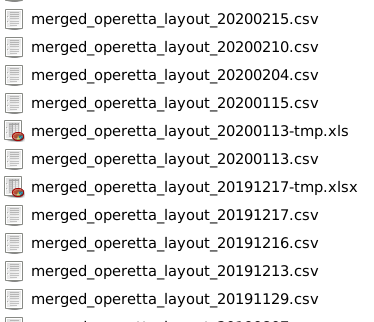
\includegraphics[height=160pt]{pictures/Screenshot_2020-02-25_17-47-03-ugly_folder-zoom_in.png}

\end{frame}

\begin{frame}

\begin{itemize}
\item the state of the art solution
\begin{itemize}
\item  have one file in the working directory
\item store the old versions 'hidden' in a \textbf{repository}
\end{itemize}
\pause
\item What is a \textbf{repository}?
\begin{itemize}
\item  a simple subfolder 
\item The folder name is '.git'.
\item It is a hidden forlder
\item You have to start git to see the content
 
\end{itemize}


\end{itemize}

\end{frame}




\begin{frame}
\frametitle<presentation>{Prediction Power VS. Difficulty of the model}
\includegraphics[height=160pt]{figures/prediction_porwer-vs-difficulty.jpg}
\end{frame}



\begin{frame}
\frametitle<presentation>{Prediction Quality}


Only the numeric columns $R^2 =0.32$

Numeric + dummy columns $R^2 =0.3302$

Only the factors $R^2 =0.2779$

Numeric+ factors $R^2 =0.4121$

numeric+dummy+ factors $R^2 =0.4192$

Transformed Data Added: $R^2 = 0.7126$

\end{frame}


\begin{frame}

R packeges for Lasso \& elastic net regression.
\begin{itemize}

\item glmnet

\item LARS (Least Angle Regression, Lasso and Forward Stagewis)
\end{itemize}

\end{frame}

\end{document}
